\newpage{}

\hypertarget{a001---duration-per-word}{%
\section{A001 - Duration per Word}\label{a001---duration-per-word}}

\hypertarget{description}{%
\subsection{Description}\label{description}}

Let us dive in with a very very simple algorithm. In fact it is the
first algorithm I tought of.

Let's say we have a task. May it read ``Buy a big book and put it in the
shelf''. And this takes a certain amount of time.

\begin{verbatim}
AmountOfTime = "Buy a big book and put it in the shelf"
\end{verbatim}

Ok, I know, language doesn't really work like that. But lets us play
stupid right now. We just split the thing into words and distribute the
duration equally to each word. The sentence above is 10 words long, so
each word gets a tenth of AmountOfTime associated with it.

Now we have a minimal time table.

We can now take another input, like ``Buy a small book''.

We know the durations associated with ``Buy'', ``a'' and ``book''. We
will have to do something about the unknown word. Ignore it, or add 10\%
to the sum of the known durations. Something like that. And voilà, we
have a time estimate.

Funny thing:

It is actually quite reasonable for the time being, that, in the absence
of further information, assigning half the duration to each subtask is
not the most stupid thing one could do.

And it is actually quite reasonable to think that buying a small book is
about the effort of buying a big one. But that is just the example.

Anyways, we now have a time estimate and noone got hurt.

\hypertarget{using-the-algorithm-from-powershell}{%
\subsection{Using the algorithm from
powershell}\label{using-the-algorithm-from-powershell}}

The algorithm is added to EstimatePS, see
Source/experiments/duration-per-word/experiment1.ps1 for a complete
example with learning, caching and usage.

Finally it is as easy as:

\begin{verbatim}
$inSeconds = Get-DPWEstimate -Model $model -DurationInSecondsFor "add a new bookkeeping api" -ProbabilityInPercent 95
\end{verbatim}

\hypertarget{how-good-is-it}{%
\subsection{How good is it?}\label{how-good-is-it}}

As you can see there is a parameter in the algorithm, the ``probability
in percent'' which decides if it should tend to higher values or not.
Since it has influence and we want to know what that influence looks
like I will use three different values for this validation: 25\%, 50\%
and 75\%.

\begin{figure}
\centering
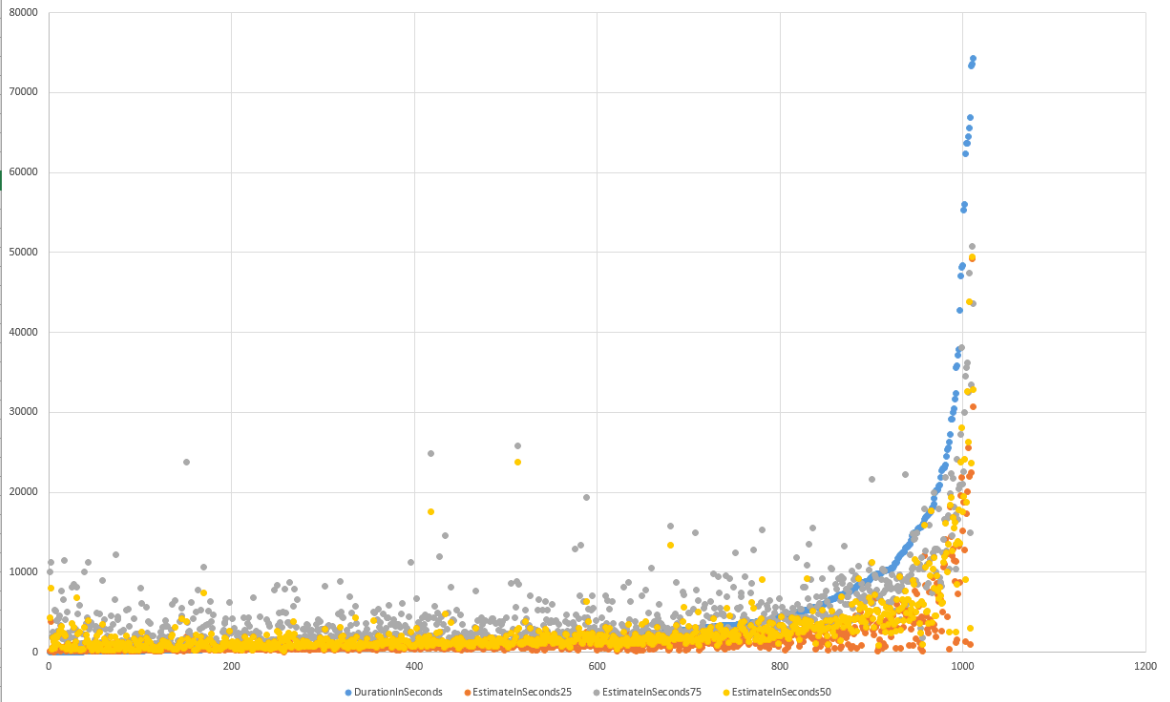
\includegraphics{Documentation/10000-A001/a001-swe2020.png}
\caption{QA a001 - swe 2020}
\end{figure}

\begin{longtable}[]{@{}lll@{}}
\toprule
Probability & Mean squared error & Percent guesses above real
duration\tabularnewline
\midrule
\endhead
25\% & 46.205.433 & 20,96\%\tabularnewline
50\% & 35.826.104 & 51,33\%\tabularnewline
75\% & 28.595.545 & 76,75\%\tabularnewline
\bottomrule
\end{longtable}

Our target mean squared error is 324.000.000 One hour is about 12.9 mio
square seconds. Two hours is about 51.8 mio square seconds. That means
that our error marin is about two hours here.

But this is the data we trained the model on, the 2020 tasks below
100000 seconds (which trims off only 12 tasks from more than 1000).

Now let us see how it performs on the 2021 tasks below 100000 seconds:

\begin{figure}
\centering
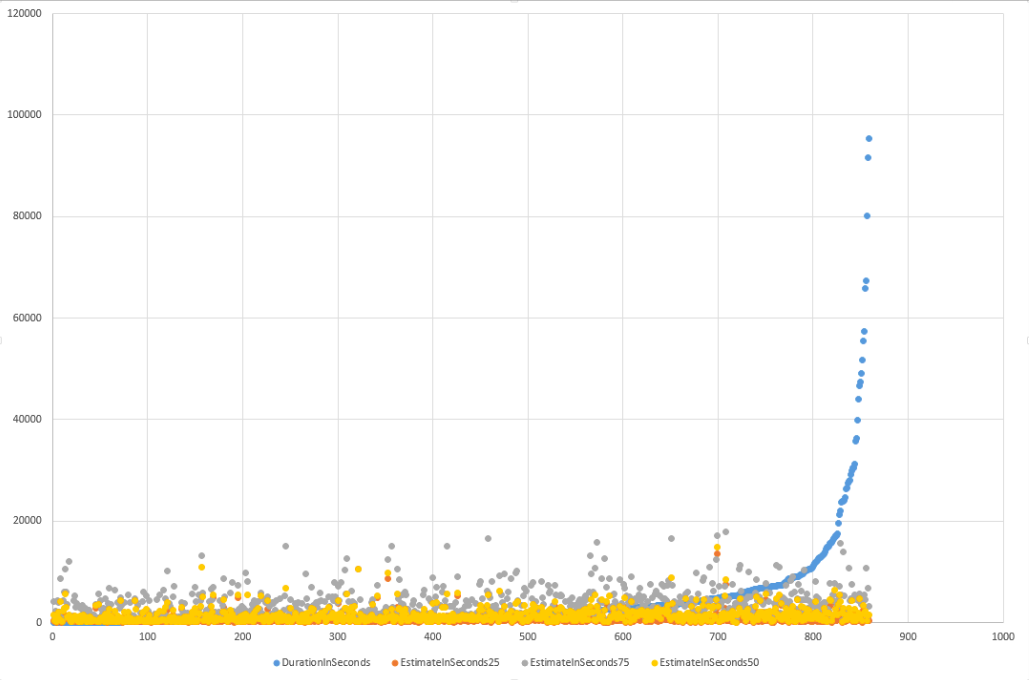
\includegraphics{Documentation/10000-A001/a001-swe2021.png}
\caption{QA a001 - swe 2021}
\end{figure}

\begin{longtable}[]{@{}lll@{}}
\toprule
Probability & Mean squared error & Percent guesses above real
duration\tabularnewline
\midrule
\endhead
25\% & 88.106.182 & 25,96\%\tabularnewline
50\% & 84.227.983 & 45,52\%\tabularnewline
75\% & 80.881.803 & 70,20\%\tabularnewline
\bottomrule
\end{longtable}

We are still below our 5h target which makes the algorithm still
acceptable, although the error margin is higher now.
